% !TEX root = mythesis.tex

%==============================================================================
\chapter{Methods}
\label{sec:methods}
%==============================================================================


\section{Hybrid Monte Carlo}
% MCMC
%% Why these algos are better that a MC
%% Markov chain definition
%%% Stationary distribution
%%% Detailed balance
% Hamiltonian Dynamics
%% Leapfrog integrator
% Metropolis Hastings
% Summary of the algo
The Hybrid (Hamiltonian) Monte Carlo (HMC) algorithm is the workhorse of modern Lattice QCD simulations and other Hamiltonian theories. This is due to the difficulty of simulating fermions with their anti-commuting nature using standard Monte Carlo (MC) methods. The major advantage of HMC over other methods is that this algorithm updates the system globally instead of the local updates that standard MC methods use. Moreover, the method is exact, meaning it does not have and truncation errors and the ensemble averages do not depend on the integration step size. These two advantages reduce the critical slowing down from which the other MC methods suffer. In the following subsections we will discuss in some detail the individual methods and algorithms that are involved in the creation of HMC.

\subsection{Markov Chain Monte Carlo}

Monte Carlo algorithms in general are used in quantum field theory to calculate the expectation value of an observable, leveraging the law of large numbers

\begin{equation}
    \langle\mathcal{O}\rangle = \frac{1}{Z} \int d\phi \mathcal{O} e^{-S[\phi]},
\end{equation}
where
\begin{equation}
    Z = \int d\phi e^{-S[\phi]}
\end{equation}
This is done by sampling $\phi$ fields from a distribution
\begin{equation}
    P(\phi) = \frac{1}{Z} \int d\phi e^{-S[\phi]}
\end{equation}
and then calculating the average
\begin{equation}
    \overline{\mathcal{O}} \equiv \frac{1}{N}\sum^{N}_{n=1} \mathcal{O}(\phi_n)
    \label{eq:ensamble_average}
\end{equation}
And in the limit of $N \to \infty$, we get the relation
\begin{equation}
    \overline{\mathcal{O}} = \langle\mathcal{O}\rangle + \mathrm{O}(1/\sqrt{N})
\end{equation}

Making simulations by sampling directly from distributions could prove very costly and practically impossible. This is because the phase space of the target distribution might be too big to explore it all (curse of dimensionality). A much better way to explore the phase space is by progressively uncovering the regions of interest, which could be done by the use of Markov Chain.

The Markov Chain is defined as a sequence of random variables $X_n$, where every next element is generated from the previous element in the chain by a transition matrix $P_{ii+1}$
\begin{equation}
    X_0 \xrightarrow{P_{01}} X_1 \xrightarrow{P_{12}} X_2 \xrightarrow{P_{23}} \cdots \xrightarrow{P_{n-1n}} X_n
\end{equation}
If the chain is ergodic and positive recurrent, then the detailed balance condition ensures that the Markov chain converges to a unique stationary distribution $p$
\begin{equation}
    p(X_i) P_{ij} = p(X_j) P_{ji}
\end{equation}

All Monte Carlo algorithm that use this method of random variable sampling are called Markov Chain Monte Carlo (MCMC) algorithms. HMC is a MCMC algorithm since we use a Markov chain to explore the target distribution, from which we draw the $\phi$ fields.

\subsection{Hamilton Dynamics}

The proposed updates to the system that we work with, must not change the energy. This is exactly what the Hamilton dynamics do, they preserve the Hamiltonian (the energy of the system). Therefore, we define Hamiltonian dynamics to evolve our $\phi(\tau)$, where $\tau$ is an evolution parameter. We introduce conjugate momenta $\pi(\tau)$ and a Hamiltonian 
\begin{equation}
    H(\phi,\pi) \equiv \frac{1}{2}\pi^2 + S(\phi),
\end{equation}
where $S(\phi)$ is the action. Now, can use the equations of motion to evolve $\phi$
\begin{equation}
    \dot{\phi} = \frac{\delta H}{\delta \pi} \qquad \dot{\pi} = - \frac{\delta H}{\delta \phi} = - \frac{\delta S}{\delta \phi}
    \label{eq:eom}
\end{equation}
The initial momentum $\pi$ is selected from a Gaussian distribution function with mean zero and unit variance. Then the whole system is evolved though the ($\phi,\pi$)-phase space. There are a lot of algorithms that can be used to solve (\ref{eq:eom}) but the most common method is the Leapfrog integrator. It is reversible and preserves the area which makes it a perfect candidate, due to the detailed balance requirement. The algorithm is simple; with initial half-step
\begin{equation}
    \pi\left(\frac{\delta\tau}{2}\right) = \pi\left(0\right) - \left[ \frac{\delta S(0)}{\delta\phi} \right] \frac{\delta\tau}{2}
\end{equation}
This is followed by $n=\frac{\tau_0}{\delta\tau}$ steps in $\phi$ and $n-1$ in $\pi$
\begin{equation}
    \begin{aligned}
        \phi(\tau+\delta\tau) = \phi(\tau) + \pi(\tau+\frac{\delta\tau}{2})\delta\tau
        \\
        \pi(\tau+\frac{\delta\tau}{2}) = \pi(\tau-\frac{\delta\tau}{2}) - \left[ \frac{\delta S(\tau)}{\delta\phi} \right] \delta\tau
    \end{aligned}
\end{equation}
and again half-step in $\pi$
\begin{equation}
    \pi(\tau_0) = \pi(\tau_0-\frac{\delta\tau}{2}) - \left[ \frac{\delta S(\tau_0)}{\delta\phi} \right] \frac{\delta\tau}{2}
\end{equation}
On Figure \ref{fig:leapfrog} is show a schematic view of the leapfrog integration process.
\begin{figure}[htbp]
    \centerline{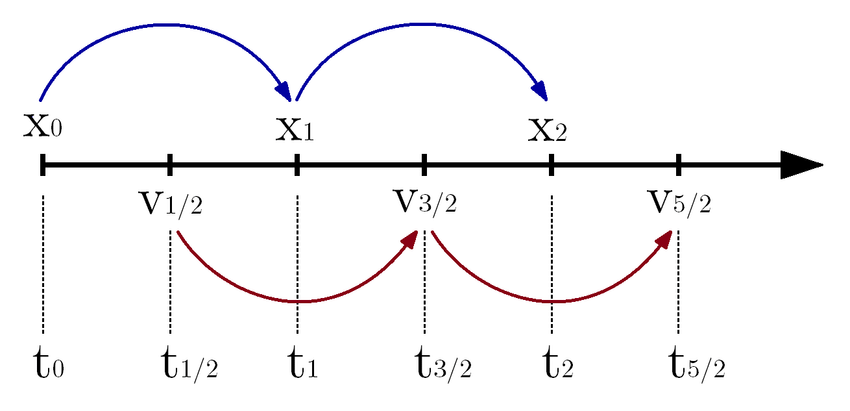
\includegraphics[width=0.5\linewidth]{leapfrog.png}}
    \caption{Leapfrog integration process. The scheme represents one integration trajectory. On each step of evolution, one of the variables lead the other by a half step, and they update each other. %https://www.researchgate.net/figure/Schematics-describing-how-the-leapfrog-algorithm-works-Position-and-velocity-leap-each_fig1_346972792}
    }
    \label{fig:leapfrog}
\end{figure}

\subsection{Metropolis-Hastings}

A Metropolis-Hastings accept/reject algorithm is used to construct a Markov chain with a stationary distribution $p(X)$. This is done by having a candidate element with transition probability $P_{acc}$. The accepted proposal is the new element of the chain, but if it is rejected the old element becomes the new one. This algorithm preserves the stationary distribution if the chain is irreducible.

\begin{figure}[htbp]
    \centerline{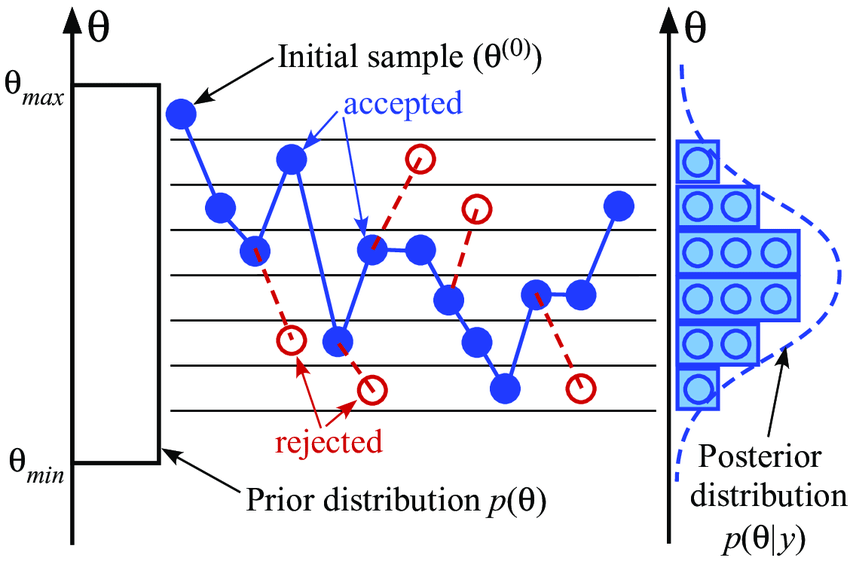
\includegraphics[width=0.5\linewidth]{
        Metropolis-Hastings-MCMC.png}}
    \caption{Metropolis-Hastings process for generating a Markov chain with a target distribution. The scheme represents the transition from an initial probability distribution to a target one. On each step, the accept/reject step is performed on the candidate element. The first element of the Markov chain is drawn from the starting distribution. The whole process is repeated until all sampled elements are representative of the new distribution. %https://www.researchgate.net/figure/Illustration-of-the-Markov-chain-Monte-Carlo-with-Metropolis-Hastings-MCMC-MH-procedure_fig6_338363810
    }
    \label{fig:mn-mcmc}
\end{figure}
This algorithm is used in HMC as an accept/reject step on the new proposed $\phi$ field. The candidate is accepted with probability 
\begin{equation}
    P_{acc} = min(1, \exp(\delta H)),
\end{equation}
where $\delta H = H' - H$ is the difference of the final and the starting Hamiltonians. This difference $\delta H$ is not zero because of the finite number of integration steps. The whole process repeats until we are satisfied by the number of configuration in the constructed Markov chain which will be averaged in (\ref{eq:ensamble_average}). On Figure \ref{fig:mn-mcmc} is shown how the Markov chain is constructed using the Metropolis-Hastings accept/reject algorithm. This acceptance rate can be tuned by the number of integration steps which can make the exploration of the phase space easier.

\subsection{Summary of the Algorithm}

We have discussed until now how we compute numerically the expectation value (\ref{eq:ensamble_average}) of an observable using MC algorithms. We also saw a better approach to draw from distributions that are difficult to sample using MCMC methods. This approach uses proposed elements which construct a Markov chain. These candidates can be found by leveraging the Hamilton dynamics and can be accepted with a probability $P_{acc}$. All of these methods culminate in the HMC algorithm, which is summarized in Algorithm (\ref{alg:hmc})

\begin{algorithm}
    \caption{Hybrid Monte Carlo}
    \begin{algorithmic}[1]
        \State Initialize  $\tau, N_{max}$
        \State Initialize $\phi_0, \pi_0$
        \State Sample $\pi_0 \sim \mathcal{N}(0,1)$

        \State Set $(\phi_{i}, \pi_{i}) = (\phi_0, \pi'_0)$ \Comment{Initial Condition}
        \While{$i < N_{max}$}  \Comment{Markov Chain}
            \State Calculate $H(\phi_{i}, \pi_{i})$
            \State Leapfrog $(\phi', \pi') \xleftarrow{\tau_\text{steps}} (\phi_{i}, \pi_{i})$ \Comment{Find a candidate}
            \State Calculate $H'(\phi',\pi')$
            \State Calculate $\delta H = H'(\phi',\pi')-H(\phi_{i},\pi_{i})$
            \If{$P_{acc} = min(1, \exp(-\delta H))$} \Comment{Accept/Reject step}
                \State Set $(\phi_{i+1}, \pi_{i+1}) = (\phi', \pi')$
                \Else
                \State Set $(\phi_{i+1}, \pi_{i+1}) = (\phi_{i}, \pi_{i})$
            \EndIf
        \State Set $i = i + 1$
        \EndWhile
    \end{algorithmic}
    \label{alg:hmc}
    \end{algorithm}
